\begin{tikzpicture}[auto,scale = 1]
		\draw (0,0) rectangle (3,3);
		\draw (3,0) rectangle (6,3);
		\node at (1.5,1.5) {$c_1$};
		\node at (4.5,1.5) {$c_2$};
		\node at (1.5,-0.3) {$s_1$};
		\node at (4.5,-0.3) {$s_3$};
		\node at (1.5,3.3) {$s_2$};
		\node at (4.5,3.3) {$s_4$};
		\node at (-0.3,1.5) {$s_5$};
		\node at (6.3,1.5) {$s_5$};
		\node at (3.3,1.5) {$s_6$};
		\node at (-0.3,-0.3) {$p_1$};
		\node at (-0.3,3.3) {$p_2$};
		\node at (6.3,3.3) {$p_1$};
		\node at (3,-0.3) {$p_3$};
		\node at (6.3,-0.3) {$p_2$};
		\node at (3,3.3) {$p_4$};
		\node at (-1.5,-1.5) {};
\end{tikzpicture}
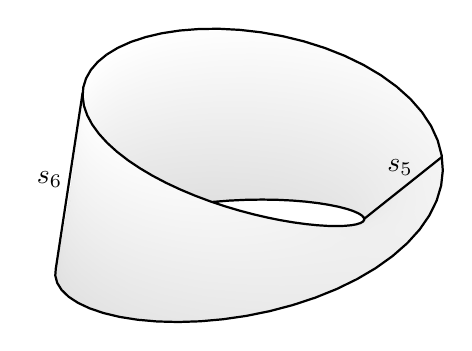
\begin{tikzpicture}

\begin{axis}[
    hide axis,
    view={40}{40}
]
\addplot3 [
    surf, shader= interp,%shader=faceted interp,
    %point meta=x,
    colormap = {whiteblack}{color(0cm)  = (gray!25);color(1cm) = (white)},
    %colormap/whiteblack,
    samples=30,
    samples y=5,
    z buffer=sort,
    domain=0:360,
    y domain=-0.5:0.5
] (
    {(1+0.5*y*cos(x/2)))*cos(x)},
    {(1+0.5*y*cos(x/2)))*sin(x)},
    {0.5*y*sin(x/2)});

\addplot3 [
    samples=50,
    domain=-140:180, % The domain needs to be adjusted manually, depending on the camera angle, unfortunately
    samples y=0,
    thick
] (
    {(1+0.5*0.5*cos(x/2)))*cos(x)},
    {(1+0.5*0.5*cos(x/2)))*sin(x)},
    {0.5*0.5*sin(x/2)});
    
    \addplot3 [
    samples=50,
    domain=-180:138, % The domain needs to be adjusted manually, depending on the camera angle, unfortunately
    samples y=0,
    thick
] (
    {(1+0.5*-0.5*cos(x/2)))*cos(x)},
    {(1+0.5*-0.5*cos(x/2)))*sin(x)},
    {0.5*-0.5*sin(x/2)});
\end{axis}

\draw[thick] (0.93,1.92) -- (1.27,4.15);
\node at (0.85,3.05) {$s_6$};
\draw[thick] (4.85,2.55) -- (5.83,3.33);
\node at (5.3,3.2) {$s_5$};

\end{tikzpicture}




